\subsection{实际工作负载下的综合评估}
\label{subsec:sgxdedup-real-world}

本文使用真实世界数据集作为测试工作负载评估\sysnameS。本文在评估中使用了以下了两个真实世界数据集\footnote{重复数据删除率的定义为原始数据容量与重复数据删除后的数据容量的比值。}:

\begin{itemize}[leftmargin=0em]
    \item \textbf{FSL数据集},包含来自文件系统和存储实验室(FSL)\cite{fsl,sun16}的共享文件系统的用户主目录的备份快照。每个快照列出了其中包含的平均大小为8\,KiB的数据块的48位指纹。本文选择了2013年1月22日至6月17日之间的在\texttt{fslhomes}目录下的所有快照,共计包含56.2\,TiB的原始数据,在重复数据删除后,数据量缩减至431.9\,GiB(即,具有133.2倍的重复数据删除率)。
    \item \textbf{MS数据集},包含来自微软公司\cite{meyer2011deduplication}的Windows文件系统快照。每个快照列出了其中包含的平均大小为8\,KiB的数据块的40位指纹。本文从原有的857个快照中选取了140个大小约为100\,GiB的快照。本文所使用的数据集包含14.4\,TiB的原始数据,在执行重复数据删除后,数据量缩减至2.4\,TiB(即,具有6倍的重复数据删除率)。
\end{itemize}

\paragraph*{Exp\#11(实际工作负载性能测试)。} 本文对\sysnameS 在真实世界数据集作为工作负载情况下的上传/下载性能进行了评估。实验从FSL和MS数据集中分别选择了10个快照。如下所示,对于FSL数据集,本文选择来自同一用户的快照以确保数据集具有较高的跨快照冗余;对于MS数据集,本文选择具有最多单个快照内冗余的10个快照。选择的FSL和MS快照分别包含1.3\,TiB和1.0\,TiB的原始数据。由于两个数据集提供的快照只包含数据块指纹等信息而不包含数据块内容,本文通过重复将其数据块指纹写入缓冲区直到达到指定的数据块大小为止来重构每个明文数据块,可确保相同(不同)指纹产生相同(不同)数据块。本文使用单个客户逐个快照进行上传,然后以与上传相同的顺序连续下载10个快照。本文将\sysnameS 与PlainDedup(Exp\#5)进行比较。

\begin{figure}[!htb]
    \centering
    \begin{tabular}{cc}
        \multicolumn{2}{c}{
\includegraphics[width=0.97\textwidth]{pic/sgxdedup/plot/exp_b2/expb2_trace_legend.pdf}} \\
        \hspace{-0.1in}
        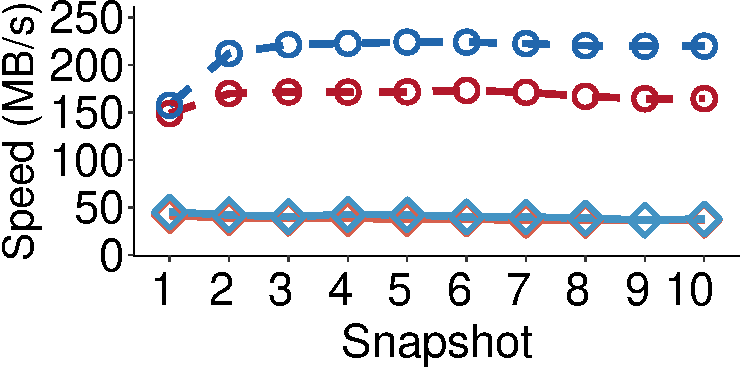
\includegraphics[width=0.47\textwidth]{pic/sgxdedup/plot/exp_b2/expb2_trace_fsl_plain_sgx.pdf} & 
        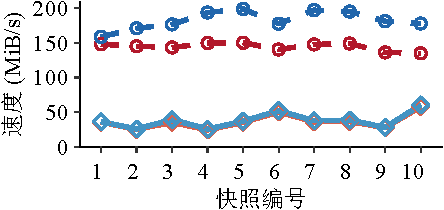
\includegraphics[width=0.47\textwidth]{pic/sgxdedup/plot/exp_b2/expb2_trace_ms_plain_sgx.pdf}               \\
        \mbox{\small (a) FSL数据集}                                                                    & 
        \mbox{\small (b) MS数据集}
    \end{tabular}
    \caption{(Exp\#11)真实世界数据集作为工作负载下的上传/下载性能}
    \label{fig:sgxdedup-tracePerformance}
\end{figure}

图~\ref{fig:sgxdedup-tracePerformance}(a)显示了所选10个FSL数据集中快照的上传/下载速度。\sysnameS 和PlainDedup都实现了很高的上传速度,尤其是在上传第一个快照时,\sysnameS 达到了148.8\,MiB/s,而PlainDedup达到了157.5\,MiB/s。原因是FSL数据集跨快照的冗余度很高,两个系统都可以为后续快照上传较少的数据。与PlainDedup相比,\sysnameS 平均会导致上传性能下降22.0\%。这里,与本文使用合成工作负载的性能评估 (Exp\#5) 相比(17.5-21.4\%),产生的性能损失略大。原因是为了重放快照中的数据块,本实验禁用了两个原型系统的数据分块模块,使得\sysnameS 的性能瓶颈转换切换到数据所有权证明(参见表~\ref{tab:sgxdedup-system-breakdown}),而PlainDedup的瓶颈是数据块指纹计算。随着下载快照的版本从旧到新,由于数据块碎片化\cite{lillibridge13}加重,\sysnameS 的下载速度从41.3\,MiB/s下降到36.4\,MiB/s,同时PlainDedup的下载速度从45.0\,MiB/s下降到37.9\,MiB/s。\sysnameS 可以通过数据块重写和缓存\cite{lillibridge13,cao2018ALACC}技术来减轻数据块碎片,提升下载性能。

图~\ref{fig:sgxdedup-tracePerformance}(b) 显示了所选10个MS数据集中快照的上传/下载速度。两个系统的上传速度都低于处理FSL数据集时的表现,这是因为MS数据集有更多的非重复数据块(MS数据集包含28.7\,M个而FSL包含18.3\,M个)加重了指纹索引的访问开销。与PlainDedup相比,\sysnameS 平均会导致21\%的上传速度下降。这里,下载速度发生显著波动(例如,\sysnameS 在24.3-57.5\,MiB/s范围内波动,而PlainDedup在25.6-60.3\,MiB/s范围内波动),这是因为某些MS快照具有更多的非重复数据块,并且可能存储在可以通过顺序读取快速访问的连续区域内(即具有更小的数据块碎片化问题\cite{lillibridge13})。

\paragraph*{Exp\#12(网络带宽开销)。} 本文评估\sysnameS 的网络带宽开销,由于\sysnameS 采用源端重复数据删除(Source-based deduplication),即客户端执行重复数据删除并仅将非重复的密文数据块上传到云服务端。因此主要对比以下三种重复数据删除方式:(1)目标端重复数据删除(Target-based deduplication),即客户端上传所有密文数据块到云服务端,云服务端对收到的密文数据块执行重复数据删除;(2)两阶段重复数据删除(Two-stage deuduplication)\cite{li15},对单个用户自身的数据执行源端重复数据删除,随后在云服务端执行目标端重复数据删除; (3)随机阈值重复数据删除(Random-threshold deduplication)\cite{harnik2010side},基于随机选择的阈值执行源端重复数据删除或目标端重复数据删除。参照\cite{harnik2010side}的默认参数,本文将随机阈值重复数据删除中选择阈值的上限和下限分别为20和2。对于FSL数据集,本文将不同用户同一天的快照聚合为单日快照,并将每个单日快照按照创建时间顺序添加到重复数据删除系统中。对于MS数据集,本文根据其快照编号由小到大添加每个快照(本文假设每个MS快照均来自不同的用户)到重复数据删除系统中。本文将实际传输数据量与原始数据量相比减少的比例定义为网络带宽节省量。这里,本文将目标端重复数据删除作为基准(传输全部数据),并且不考虑传输元数据产生的网络带宽开销。

\begin{figure}[!htb]
    \centering
    \begin{tabular}{@{\ }c@{\ }c}
        \multicolumn{2}{c}{
\includegraphics[width=0.9\textwidth]{pic/sgxdedup/plot/upload_traffic/upload_traffic_legend.pdf}} \\
        \hspace{-0.1in}
        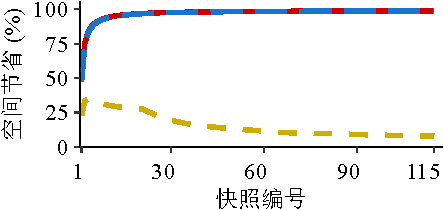
\includegraphics[width=0.47\textwidth]{pic/sgxdedup/plot/upload_traffic/upload_traffic_fsl.pdf} & 
        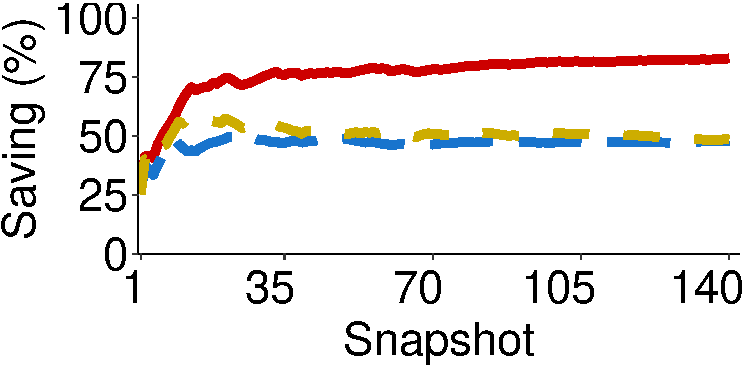
\includegraphics[width=0.47\textwidth]{pic/sgxdedup/plot/upload_traffic/upload_traffic_ms.pdf}                        \\ 
        \mbox{\small (a) FSL数据集}                                                                     & 
        \mbox{\small (b) MS数据集}
    \end{tabular}
    \caption{(Exp\#12) 存储每个快照后的累积网络带宽节省(目标端重复数据删除为基准)}
    \label{fig:sgxdedup-uploadTraffic}
\end{figure}

图~\ref{fig:sgxdedup-uploadTraffic}显示了上传每个快照后的累积带宽节省。上传所有快照后,\sysnameS 在FSL和MS数据集中分别实现了99.2\%和83.2\%的带宽节省。由于\sysnameS 执行源端重复数据删除,因此其带宽节省与存储空间节省表现一致。两阶段重复数据删除在FSL数据集中与\sysnameS 节省的带宽几乎相同,这是因为FSL数据集包含大量用户内冗余。另一方面,在MS中,两阶段重复数据删除仅节省了47.9\%的带宽(与\sysnameS 相比差异绝对值达35.3\%)。随机阈值重复数据删除对两数据集具有不同的带宽节省,在MS数据集中节省了48.5\%,但在FSL数据集中只节省了7.8\%(均小于\sysnameS,差异绝对值分别为34.7\%和91.4\%)。

